\documentclass[a4paper,10pt]{article}
\usepackage[utf8]{inputenc}
\usepackage[english]{babel}
\usepackage{indentfirst}
\usepackage{listings}
\usepackage{graphicx}
\usepackage{blindtext}
\usepackage{enumitem}
\usepackage{hyperref}
\usepackage[top=2.5cm,bottom=2.5cm,left=2.5cm,right=2.5cm]{geometry}
\pagestyle{headings}
\title{Ftp server in a datadiode}
\author{Rusu George, Boulif Ilias, Orinx Cédric}
\date{\today}

\begin{document}
\maketitle
\newpage
\tableofcontents
\newpage
\section{Concept of operations}
\subsection{Introduction to the problem}
Our client would want to prevent his research and development labs against industrial espionage and confidential information leaking. He wants to divide the company network in order to maintain the labs in an isolated environment. Thus, the critical data could not leave the company using the network. One problem related is assuring that all the operating systems are up-to-date. This could be achieved using a manual operation where an employee would manually update every node in the isolated network using a mass-storage device\footnote{A USB-key for instance.}. However, this is not the most optimized way and for sure it is not cost less and timeless for the company, without mentioning that there could be dependency problems. This method is also prone to human errors and this could generate security vulnerabilities.

\subsection{Our solution}
In order to address this problem we are going to implement a data diode. In electronics as shown in Figure \ref{fig:diode}, a diode is a component which conduct the current in one direction. Thus the term of data diode is a set of components that only let the data to travel in an unidirectional way. An example of use case is illustrated in Figure \ref{fig:datadiode}, letting the data pass from a low risk LAN to a high risk LAN but not the way around.
\begin{figure}
\centering
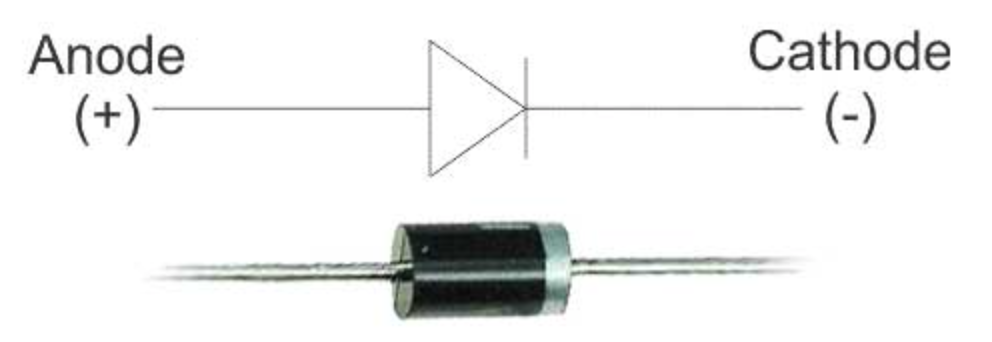
\includegraphics[scale=0.25]{images/diode.png}
\caption{A diode schema in electrionics.}
\label{fig:diode}
\end{figure}

\begin{figure}
\centering
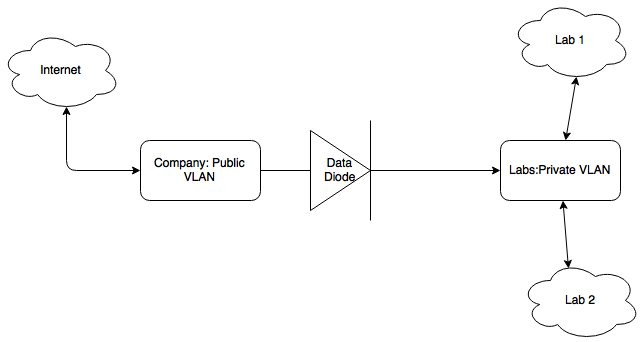
\includegraphics[scale=0.45]{images/dataDiode.png}
\caption{The schema of the usage of a data diode in a company network.}
\label{fig:datadiode}
\end{figure}

A data diode is made using one transmitter(Tx) and one receiver(Rx) both linked using only one fiber cable. Thus, when a digital data is sent through, every bit will be converted\footnote{Using a Digital-to-analog converter (DAC).} into an electrical pulse which will be convert in light pulse using a LED\footnote{Light Emitting Diode.}. Then, the output light will pass trough the fiber cable and as soon as the photons are reaching the receiver, they will be converted firstly into an electrical pulse by a photo diode and then in bits\footnote{Using an analog to digital converter (ADC).}. Since there is only one fiber, data can only travel in one way.

One major problem of this system is the network transport protocols(layer 4 in the OSI model) that applications are using. The most used transportation protocol nowadays is TCP. However, TCP is a bi-directional protocol which need the 3 way handshake in order to start a connection, thus there must be at least two fiber cables. In contradiction, UDP does not require a handshake process because it does not provide reliability, ordering, data integrity and does not set up a dedicated end-to-end connection automatically. Thus, UDP protocol does not necessary require a bi-directional data transfer. Therefore, the use of such a protocol is recommended when dealing with applications that are not sensitive to data loss or that implements an error checking system. Hence, the use of the UDP protocol within the data diode.

It seems obvious now that the transport protocol used between the transmitter and the receiver of the data diode is UDP. However, this brings multiple problems. One of the problems is how to be able to use applications that requires TCP. Another problem could be the reliability of the digital data transfer in the data diode, how can we ensure that there will not be any data loss during the transfer. We will address to those questions further down in this document.\bigskip

Furthermore, system administrators would dispose of a file transmission mechanism from the low level to the high level in order to maintain all the computers up to date. This will be done using the FTP protocol and will be explained in the next section.

\subsection{Our System description}
The data diode concept is well orchestrated combination between hardware and software. The data diode is composed of two servers: a transmitter and a receiver. We could consider that the transmitter server is connected to the low security risk LAN where a connection to the internet is made and where all the employees are connected. The receiver is connected to the high security risk LAN where all the labs are connected and where critical informations are stored.

The transmission of the information will be from the low side to the high side and blocked the way around as shown in Figure \ref{fig:UDPDD}.

\begin{figure}
\centering
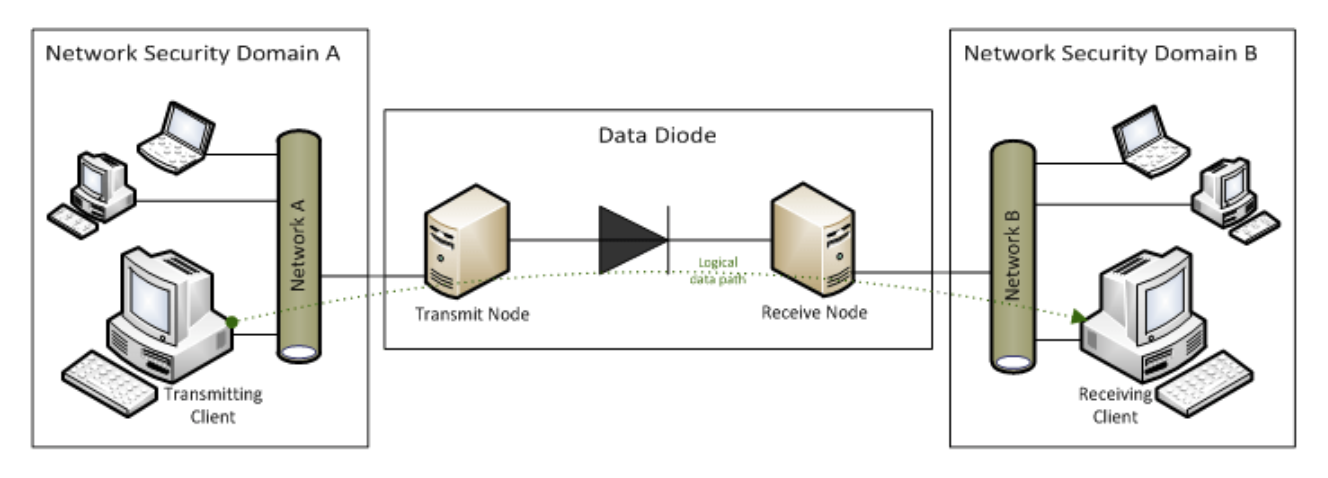
\includegraphics[scale=0.5]{images/logical-scheme-DD.png}
\caption{Data logical path within the data diode.}
\label{fig:UDPDD}
\end{figure}

\subsubsection{Hardware}
The following table presents the components used for the data diode implementation. We should mention that both transmitter and receiver possess two NICs\footnote{Network interface controller.}: one for the communication within the LAN and one for the data diode.\bigskip
\begin{table}[!h]
\centering
\begin{tabular}{|p{3cm}|p{10.5cm}|}
	\hline
	\textbf{Components} & \textbf{Description}                 \\
	\hline
	Transmitter server  &  a physical machine or a virtual machine. The NIC for the data diode will be set in transmission mode only. \\
	\hline
	Receiver server  &  a physical machine or a virtual machine. Similar to the transmission, the nic will only be set in a receiver mode.\\
	\hline
	One fiber/UTP & This optical fiber allows communication between the low server the high server. It will probably be simulated using a UTP/RJ45 cable.\\
	\hline
	4 Fiber NIC/UTP NIC & Two for each server (transmission and receiver).  \\
	\hline
\end{tabular}
\caption{Components description}
\label{tab:component}
\end{table}
\subsubsection{Software}
The Linux distribution which will be used in our project will be GNU Debian. We will have two linux machine, one on the transmitter side and one on the receiver side. 

The data diode will be easily administrated using a web interface running on an Apache server. The web site will be hosted on the transmission server. It will be described in more details further in this document.

Every configuration script used by the web interface will be a combination of Python language and Bash language.
\subsubsection{First overview on the project implementation}

Let's start by explaining which protocol shall be used in the data diode. Remember that our main goal is to create an isolated environment but also to facilitate the update process of the machines within the high security zone. As we mentioned earlier, we are going to use the FTP\footnote{File transfer protocol.} protocol. There are some alternatives to FTP such as BlindFTP, SFTP, etc. However FTP and SFTP are using TCP as their transportation layer protocol. Thus, we are going to use between the transmitter and the receiver the BlindFTP which use UDP instead.

BlindFTP is a simple Python script which was especially created for the communication between the two servers over an unidirectional network. It is simply a tool for transferring files from one side to the other. Despite the fact that use UDP, there is no acknowledgement of received packets but this is compensated by a redundancy of the data. An other advantage is the language used, as it is written in Python the result code is relatively simple and very portable to Windows or MacOS.

It is now time to have a look to our entire system, let's have a look in Figure \ref{fig:sysschem}.\bigskip

\begin{figure}
\centering
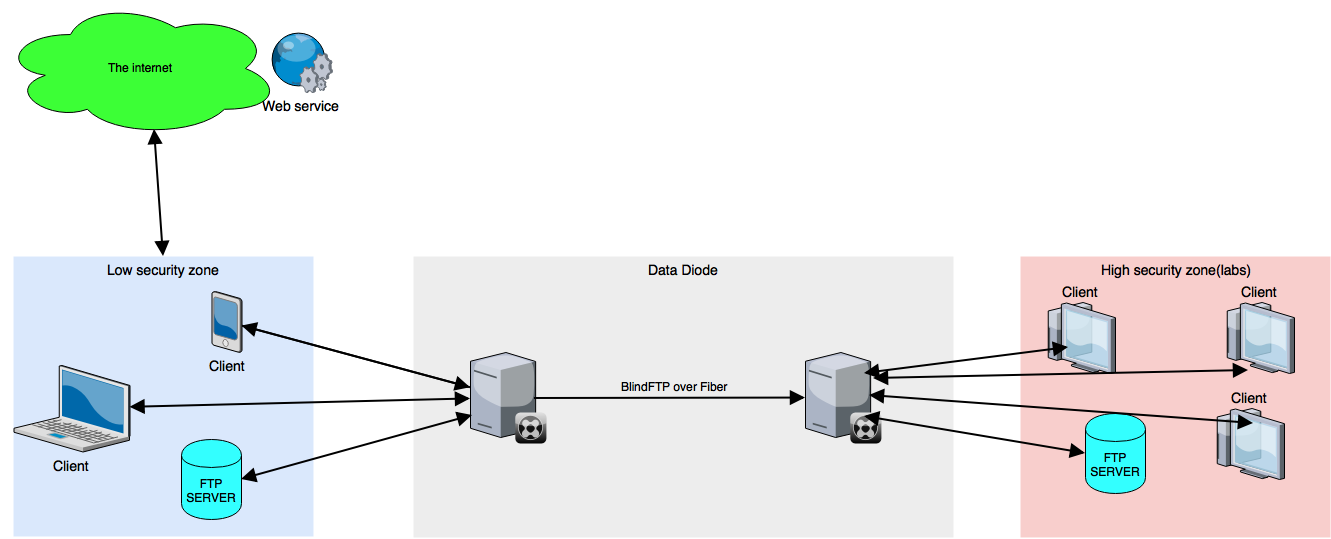
\includegraphics[scale=0.35]{images/systemschema.png}
\caption{Entire system.}
\label{fig:sysschem}
\end{figure}

Using BlindFTP allows us to ignore if the application is using TCP or UDP, the only thing we need is to make sure that the data arrive to the transmitter. We should note that between the transmitter and the other peers a TCP connection can be used to communicate. And this is the same for the receiver, after the data goes out from the network diode the transportation protocol could be TCP with other computers. In this way, we are not dealing any more with the problem of application transportation layer. 

\subsection{Users} 
In general every employee of a company has a unique ID, a grade, a job title, etc. The company owner or the manager in charge with the security could choose which grade or which person can have access to the administration web interface, of course this exclude the systems administrators.  Thus to make our explanation simple, let's suppose that there will be two types of users in our system : the \textit{administrators} and the all the other \textit{users}.

A \textit{user} is simply an employee of the company. Every employee have limited access into the company's files according to their job title or to the specific rule defined by their supervisor.

An \textit{administrator} is a user in charge of operating and maintaining the data diode. It is the only authorized person to interact with the data diode and this is mandatory. Because he will have to know how the data diode is working, should know how to interact with it using the web interface but mostly he should be able to reconfigure it or restore it as quickly as possible in case of a security breach or a system failure. However, an administrator could not have access to some strict secret files of the company but only to the used IT mechanism.

Every user information is managed and stored by the company in their own databases.

\subsection{User Interface}

As we mentioned earlier, the administration of our data diode will happen through a web interface. There will be one web interface hosted on the transmitter which will allows to transmit files or update packages from the lower network to the higher network. But, on the other hand there will also be a receiver web interface for each user to manipulate his transferred data more easily.

Each user should login from both side to use the platform. Here is an overview of our login page:

\begin{figure}[!h]
\centering
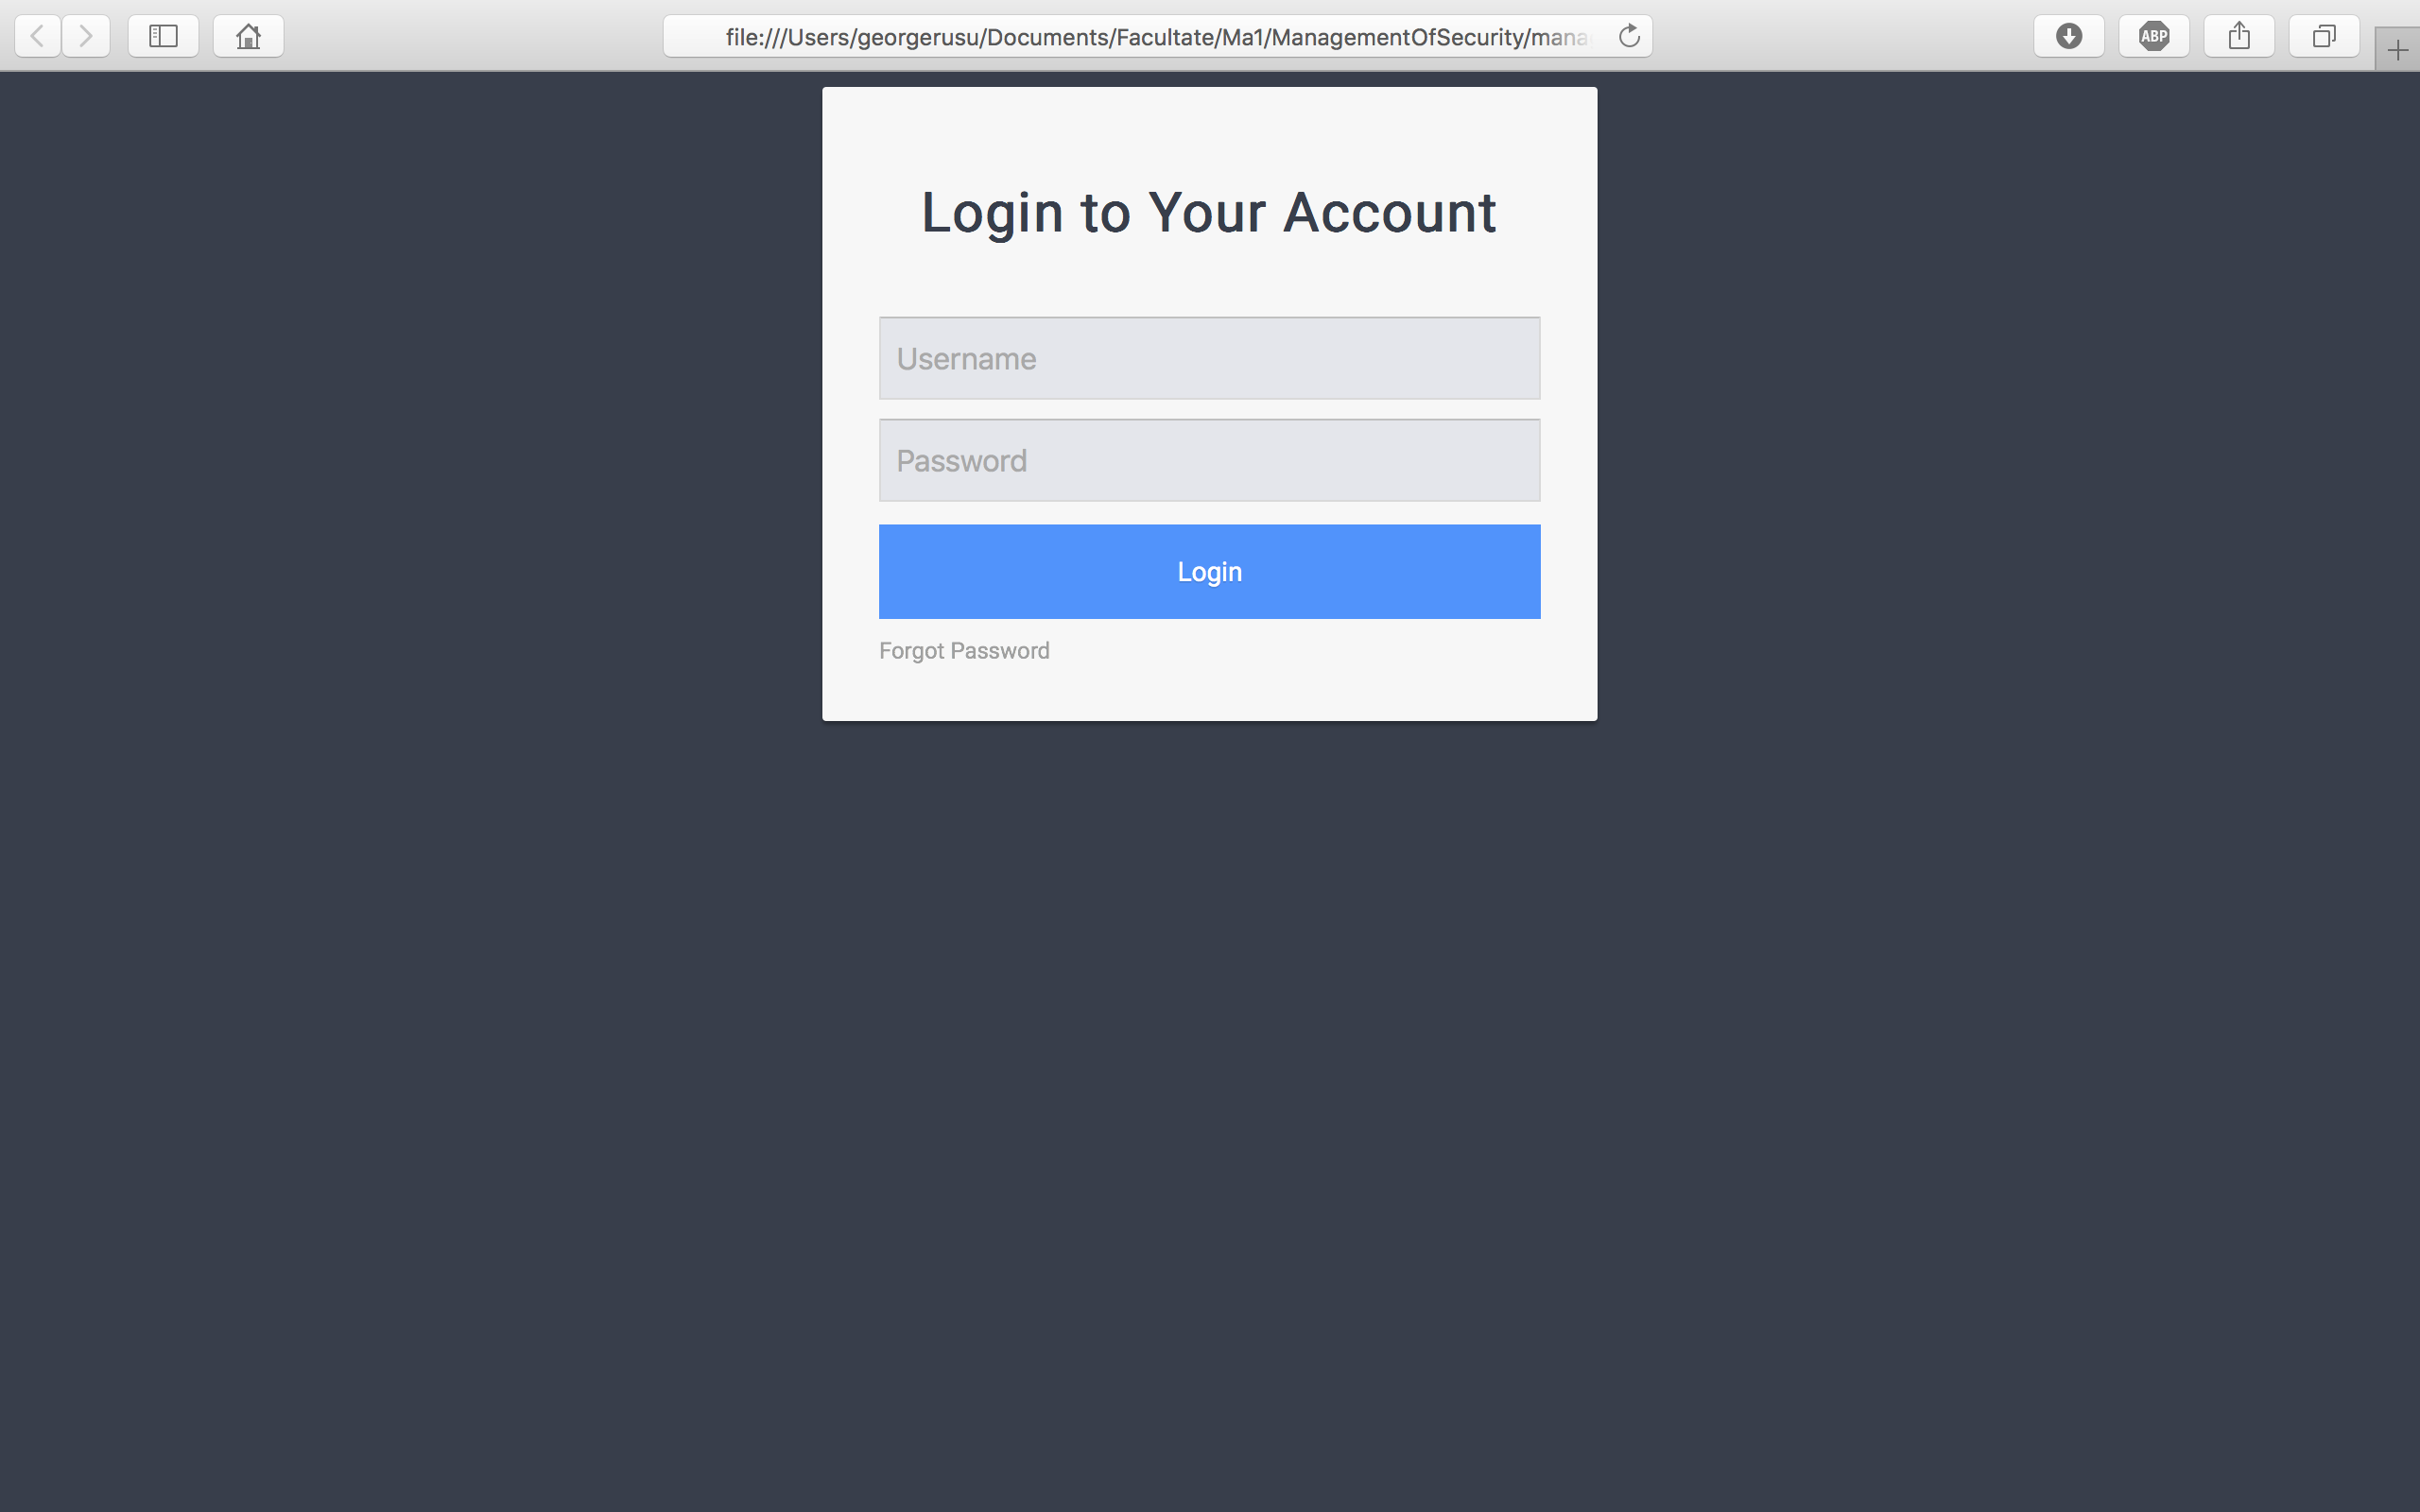
\includegraphics[scale=0.35]{images/login.png}
\caption{Login page.}
\label{fig:logpage}
\end{figure}

Once login is made, the user will be prompted to the web interface of the transmitter or the receiver. The page are shown in Figure \ref{fig:transuserpage} and Figure \ref{fig:receiveruserpage}.


\begin{figure}[!h]
\centering
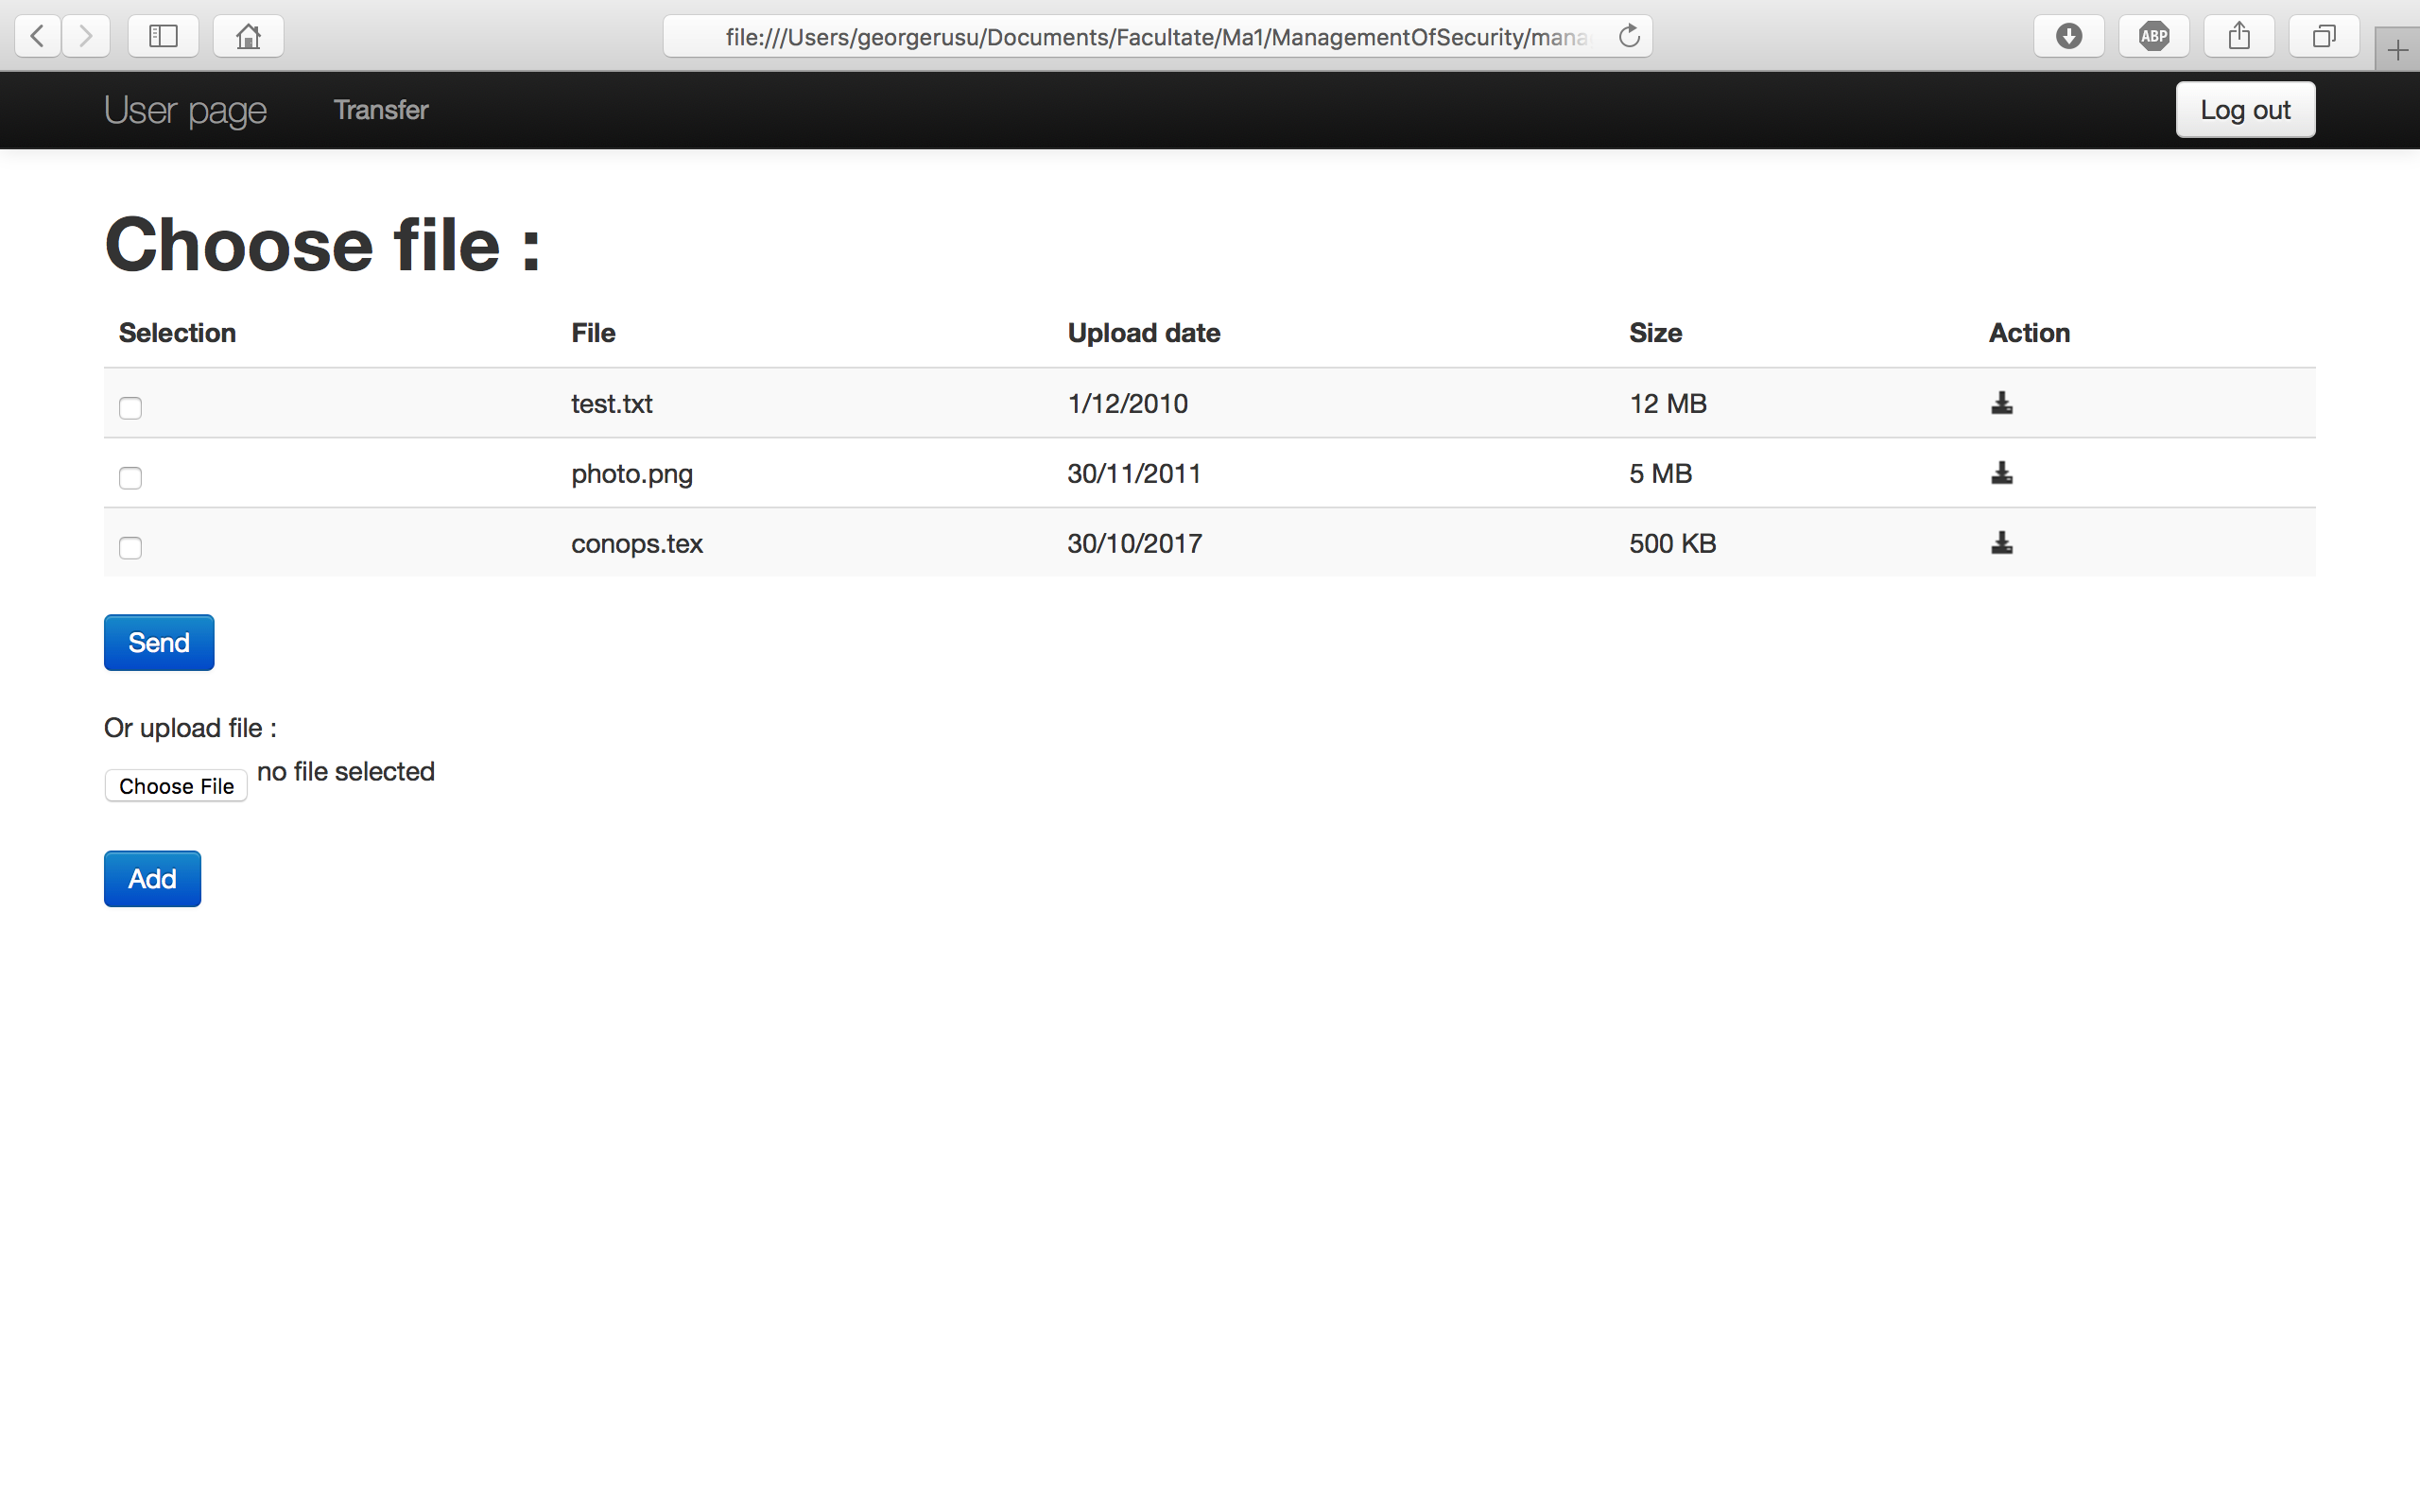
\includegraphics[scale=0.35]{images/usertransmitter.png}
\caption{Transmitter user page.}
\label{fig:transuserpage}
\end{figure}

\begin{figure}[!h]
\centering
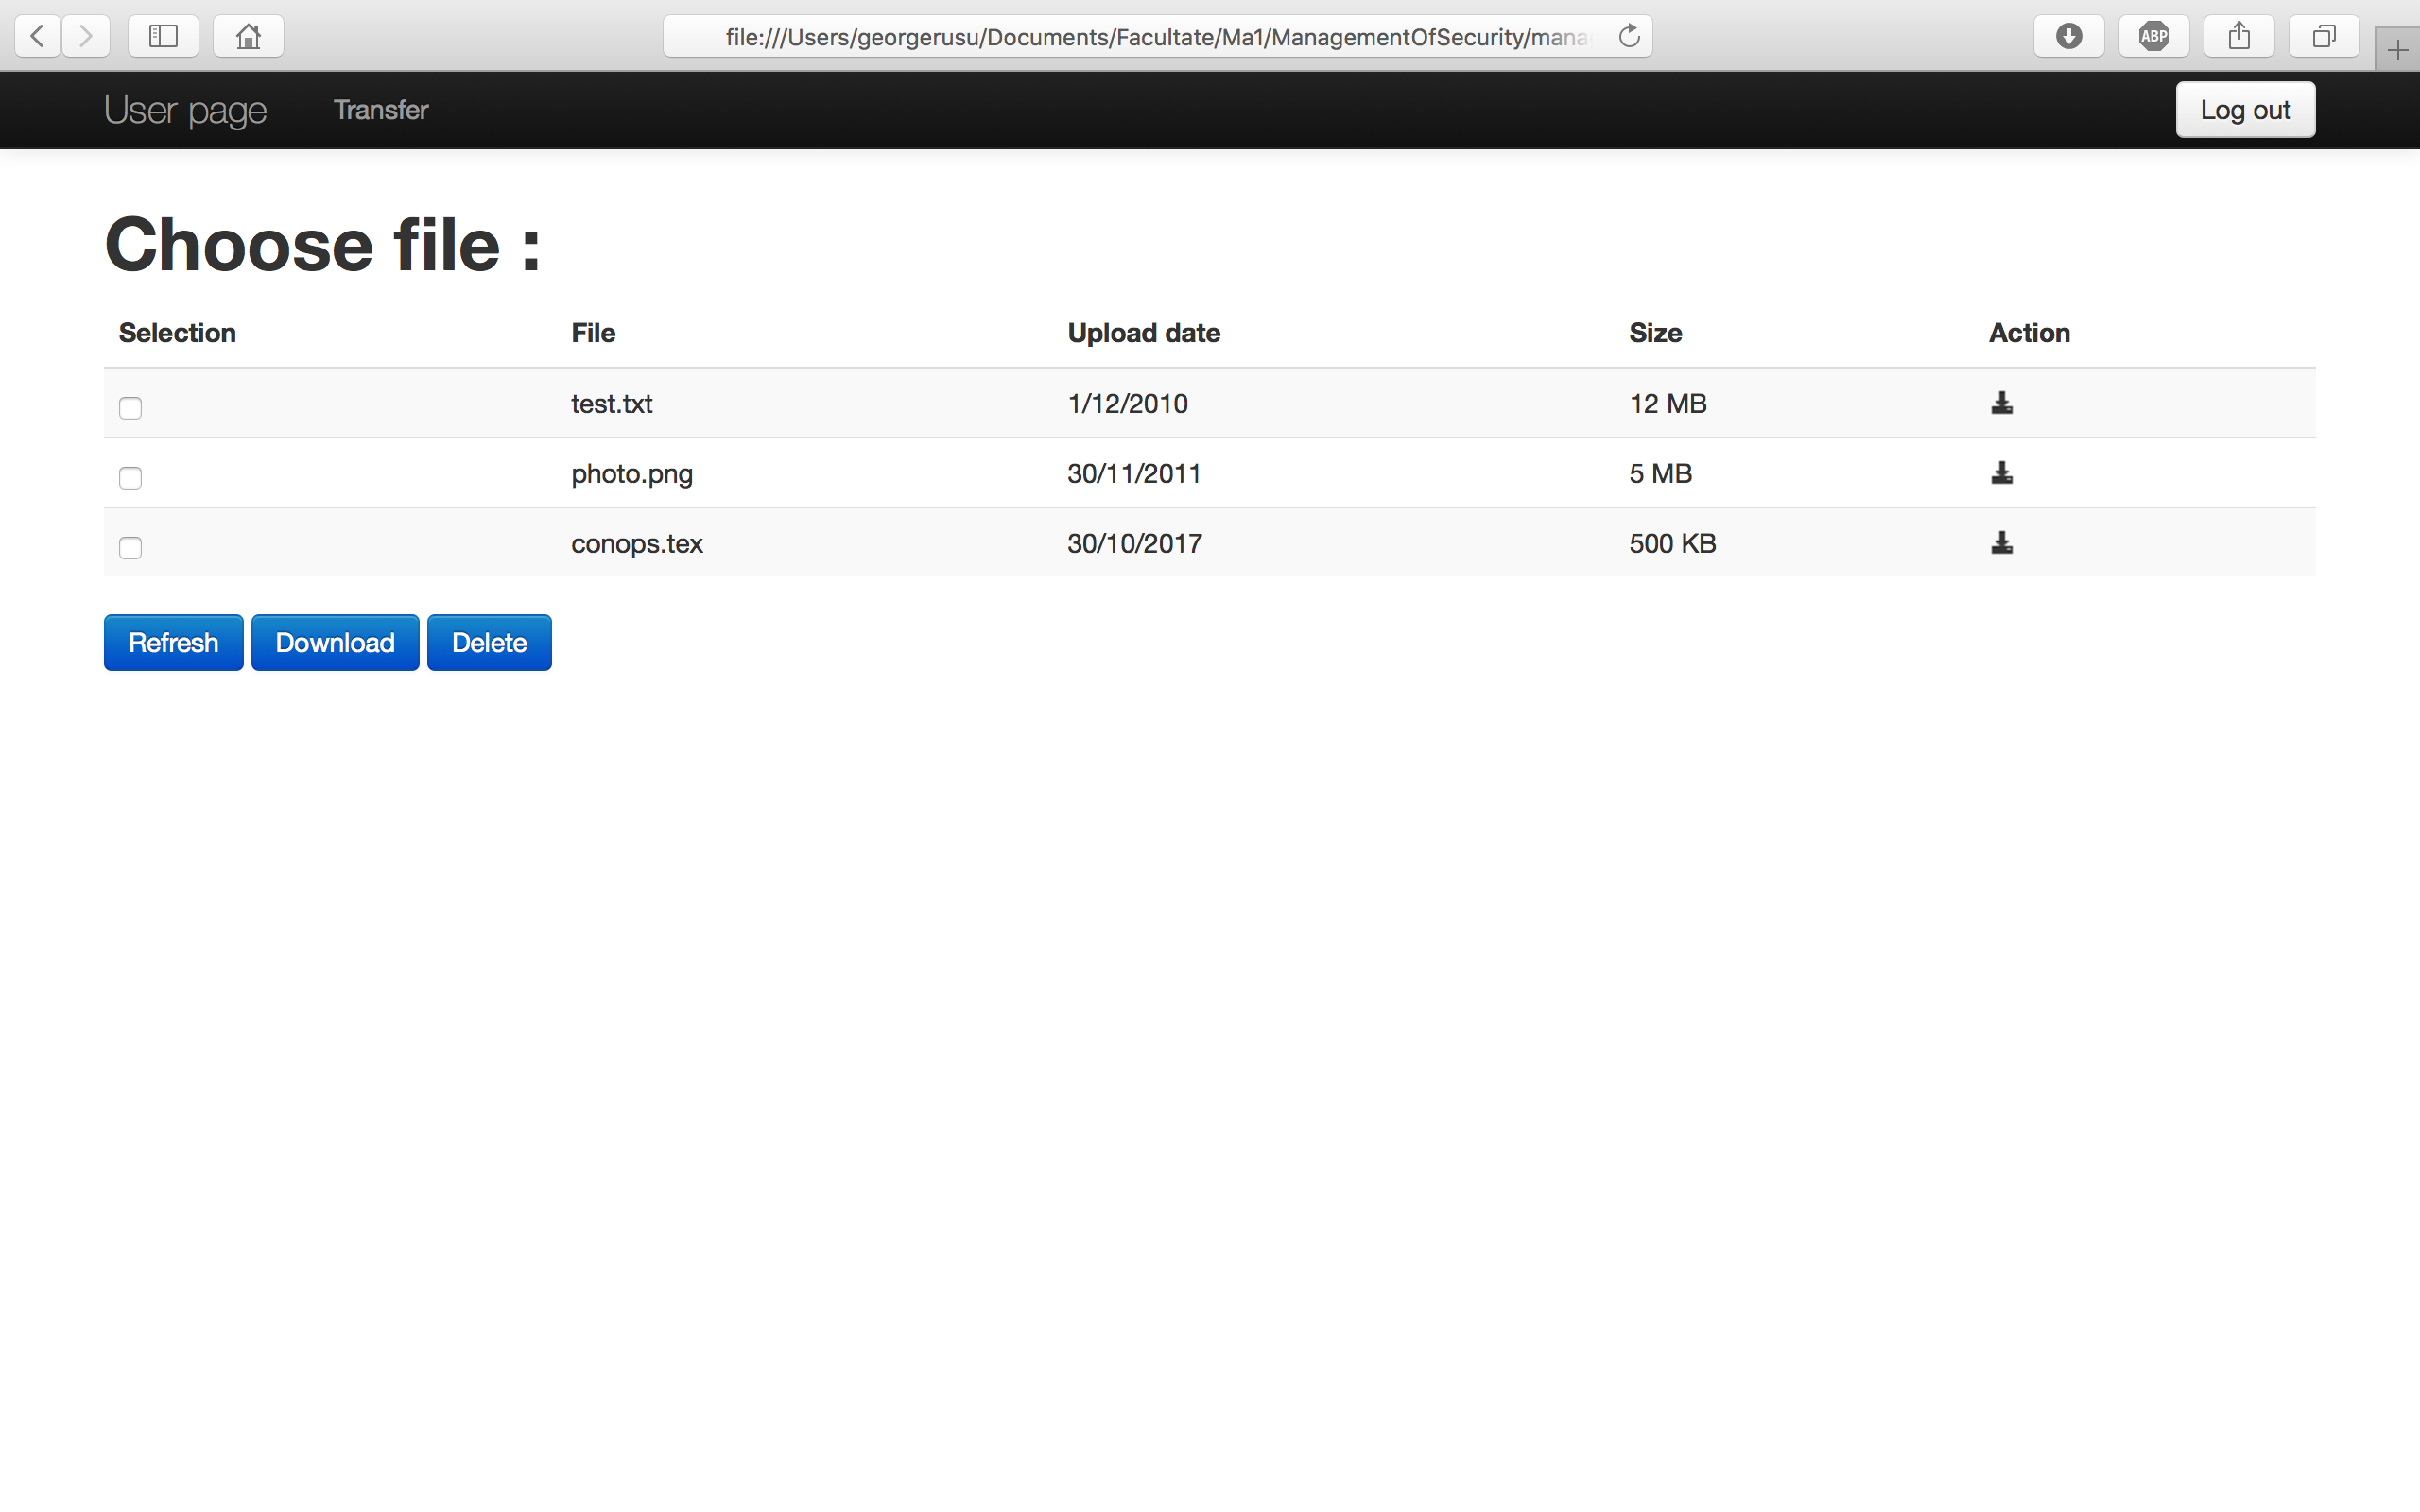
\includegraphics[scale=0.35]{images/userreceiver.png}
\caption{Receiver user page.}
\label{fig:receiveruserpage}
\end{figure}

On the other hand, an admin can transfer files but also can transfer updated packages from official sources or he can upload a package from his own PC. The admin interface is shown in Figure \ref{fig:transadminpage}
and in Figure \ref{fig:receiveradminpage}.
\begin{figure}[!h]
\centering
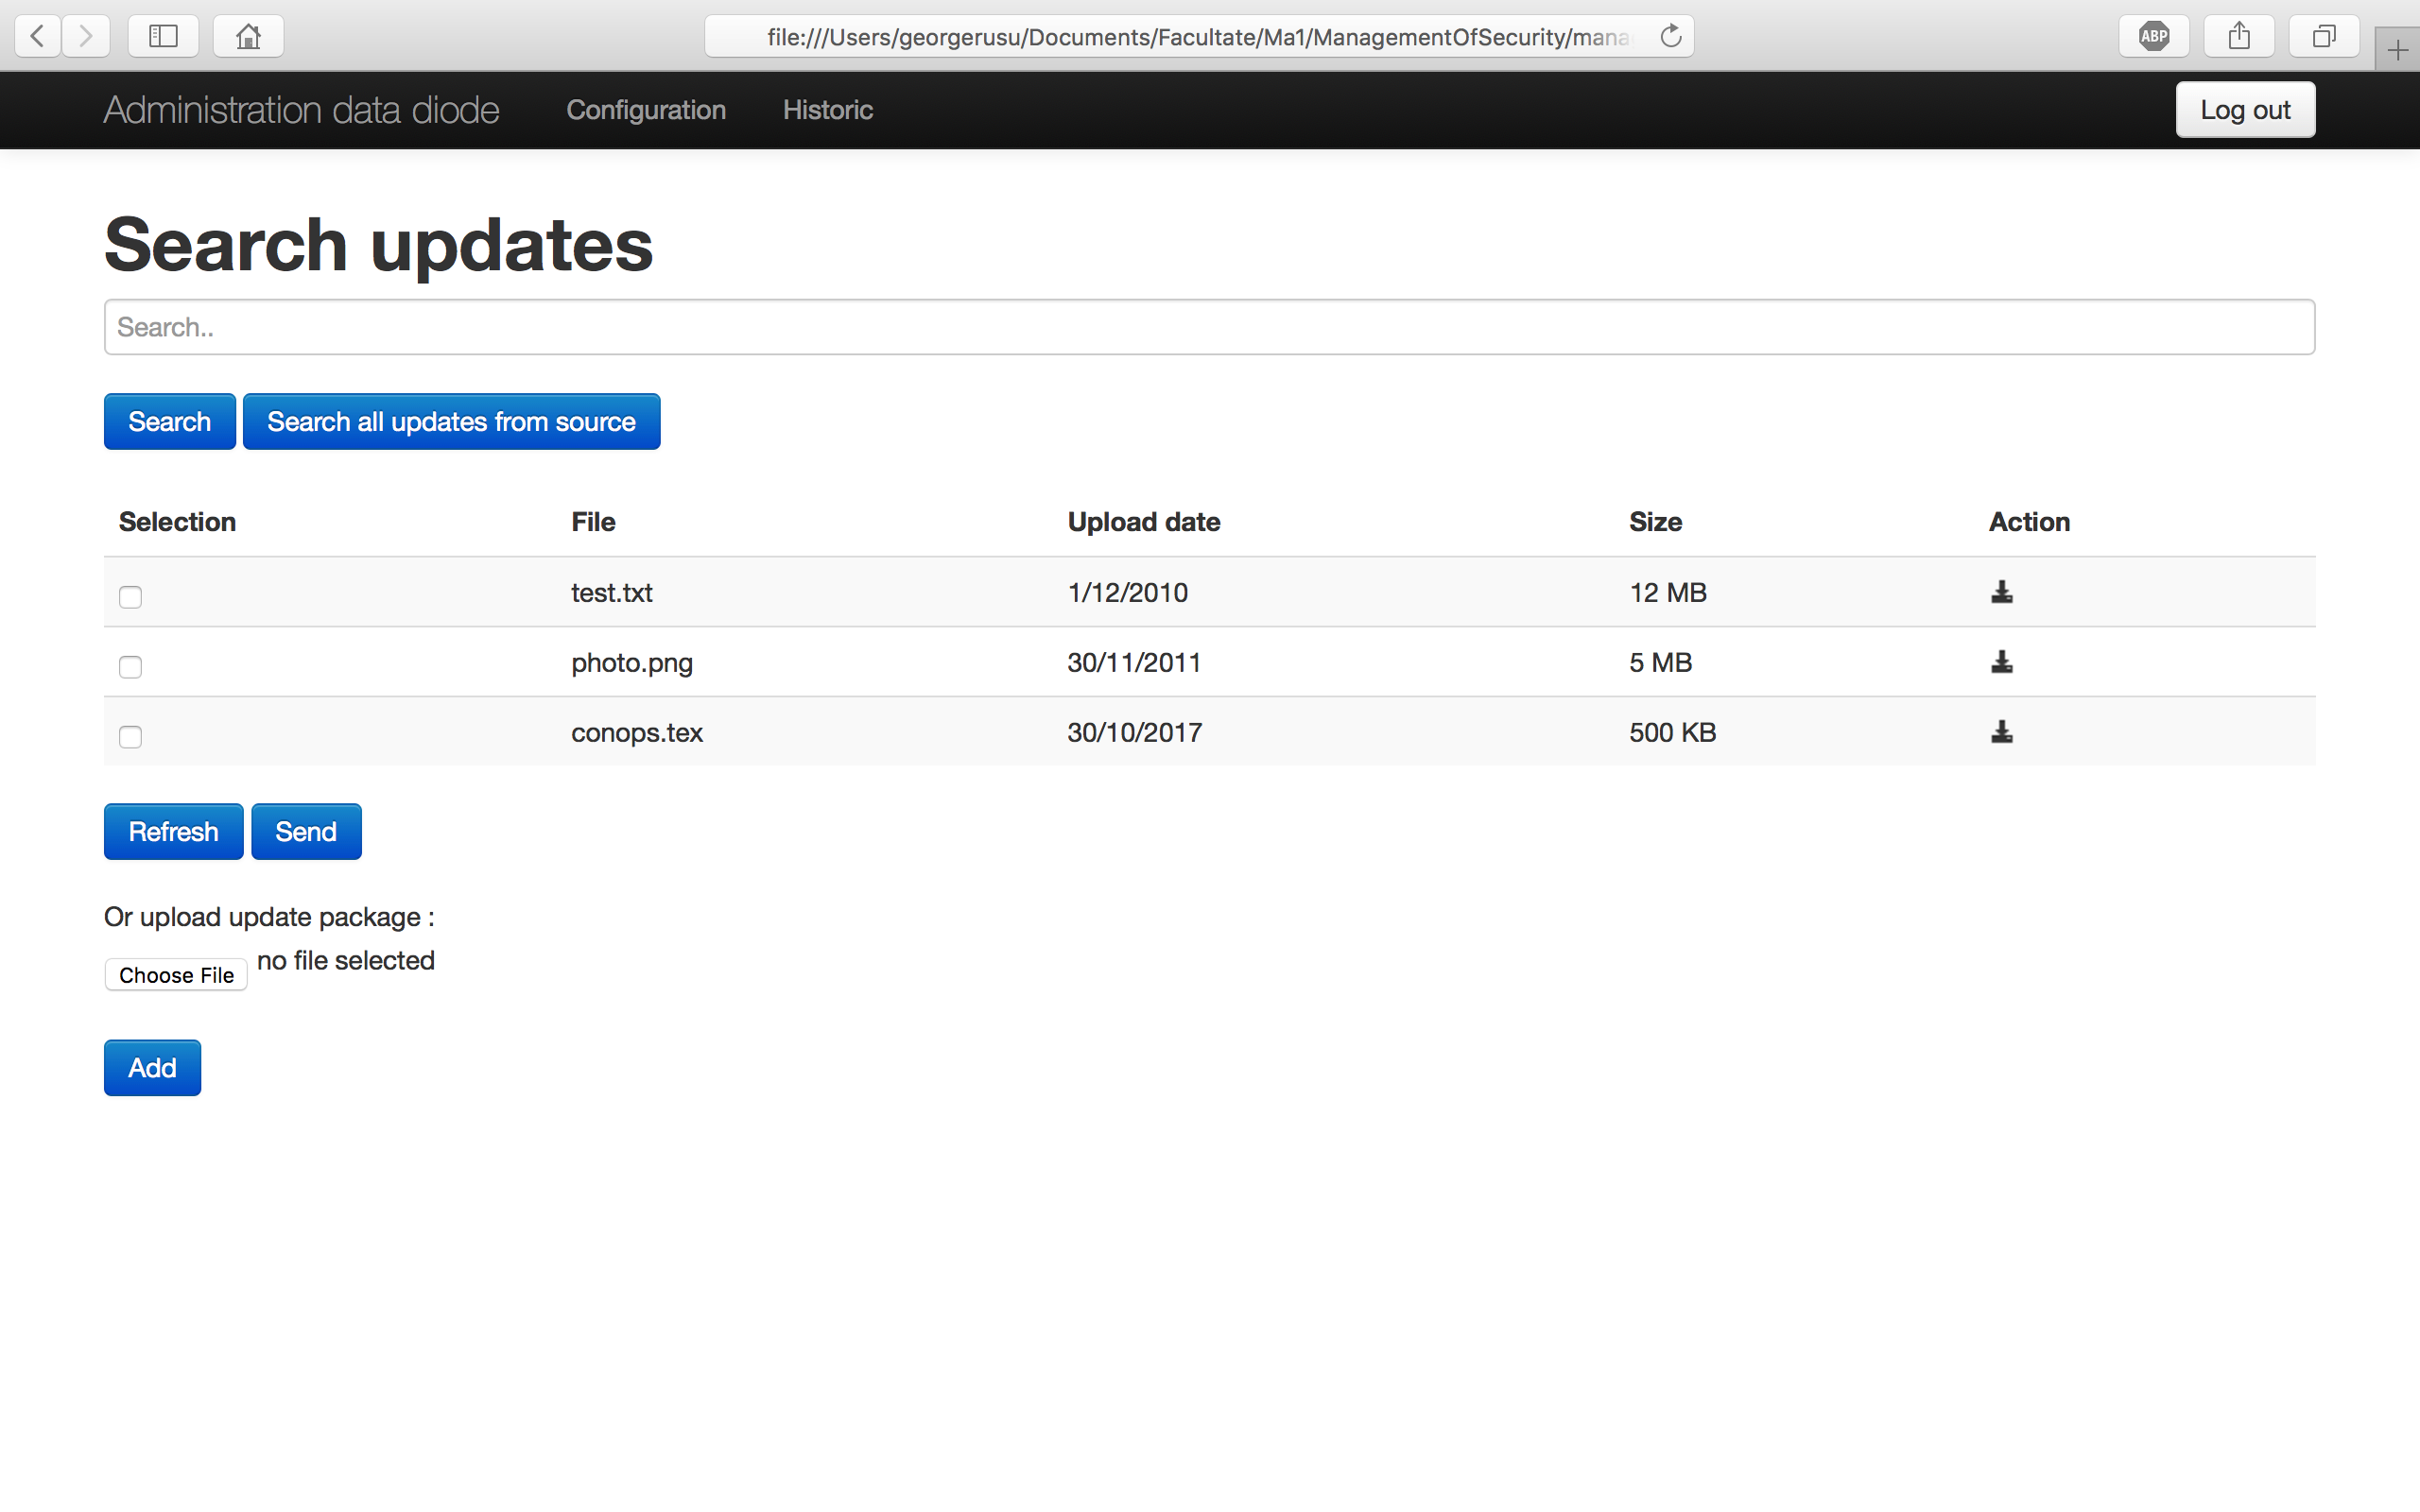
\includegraphics[scale=0.35]{images/admintransmitter.png}
\caption{Transmitter admin page.}
\label{fig:transadminpage}
\end{figure}

\begin{figure}[!h]
\centering
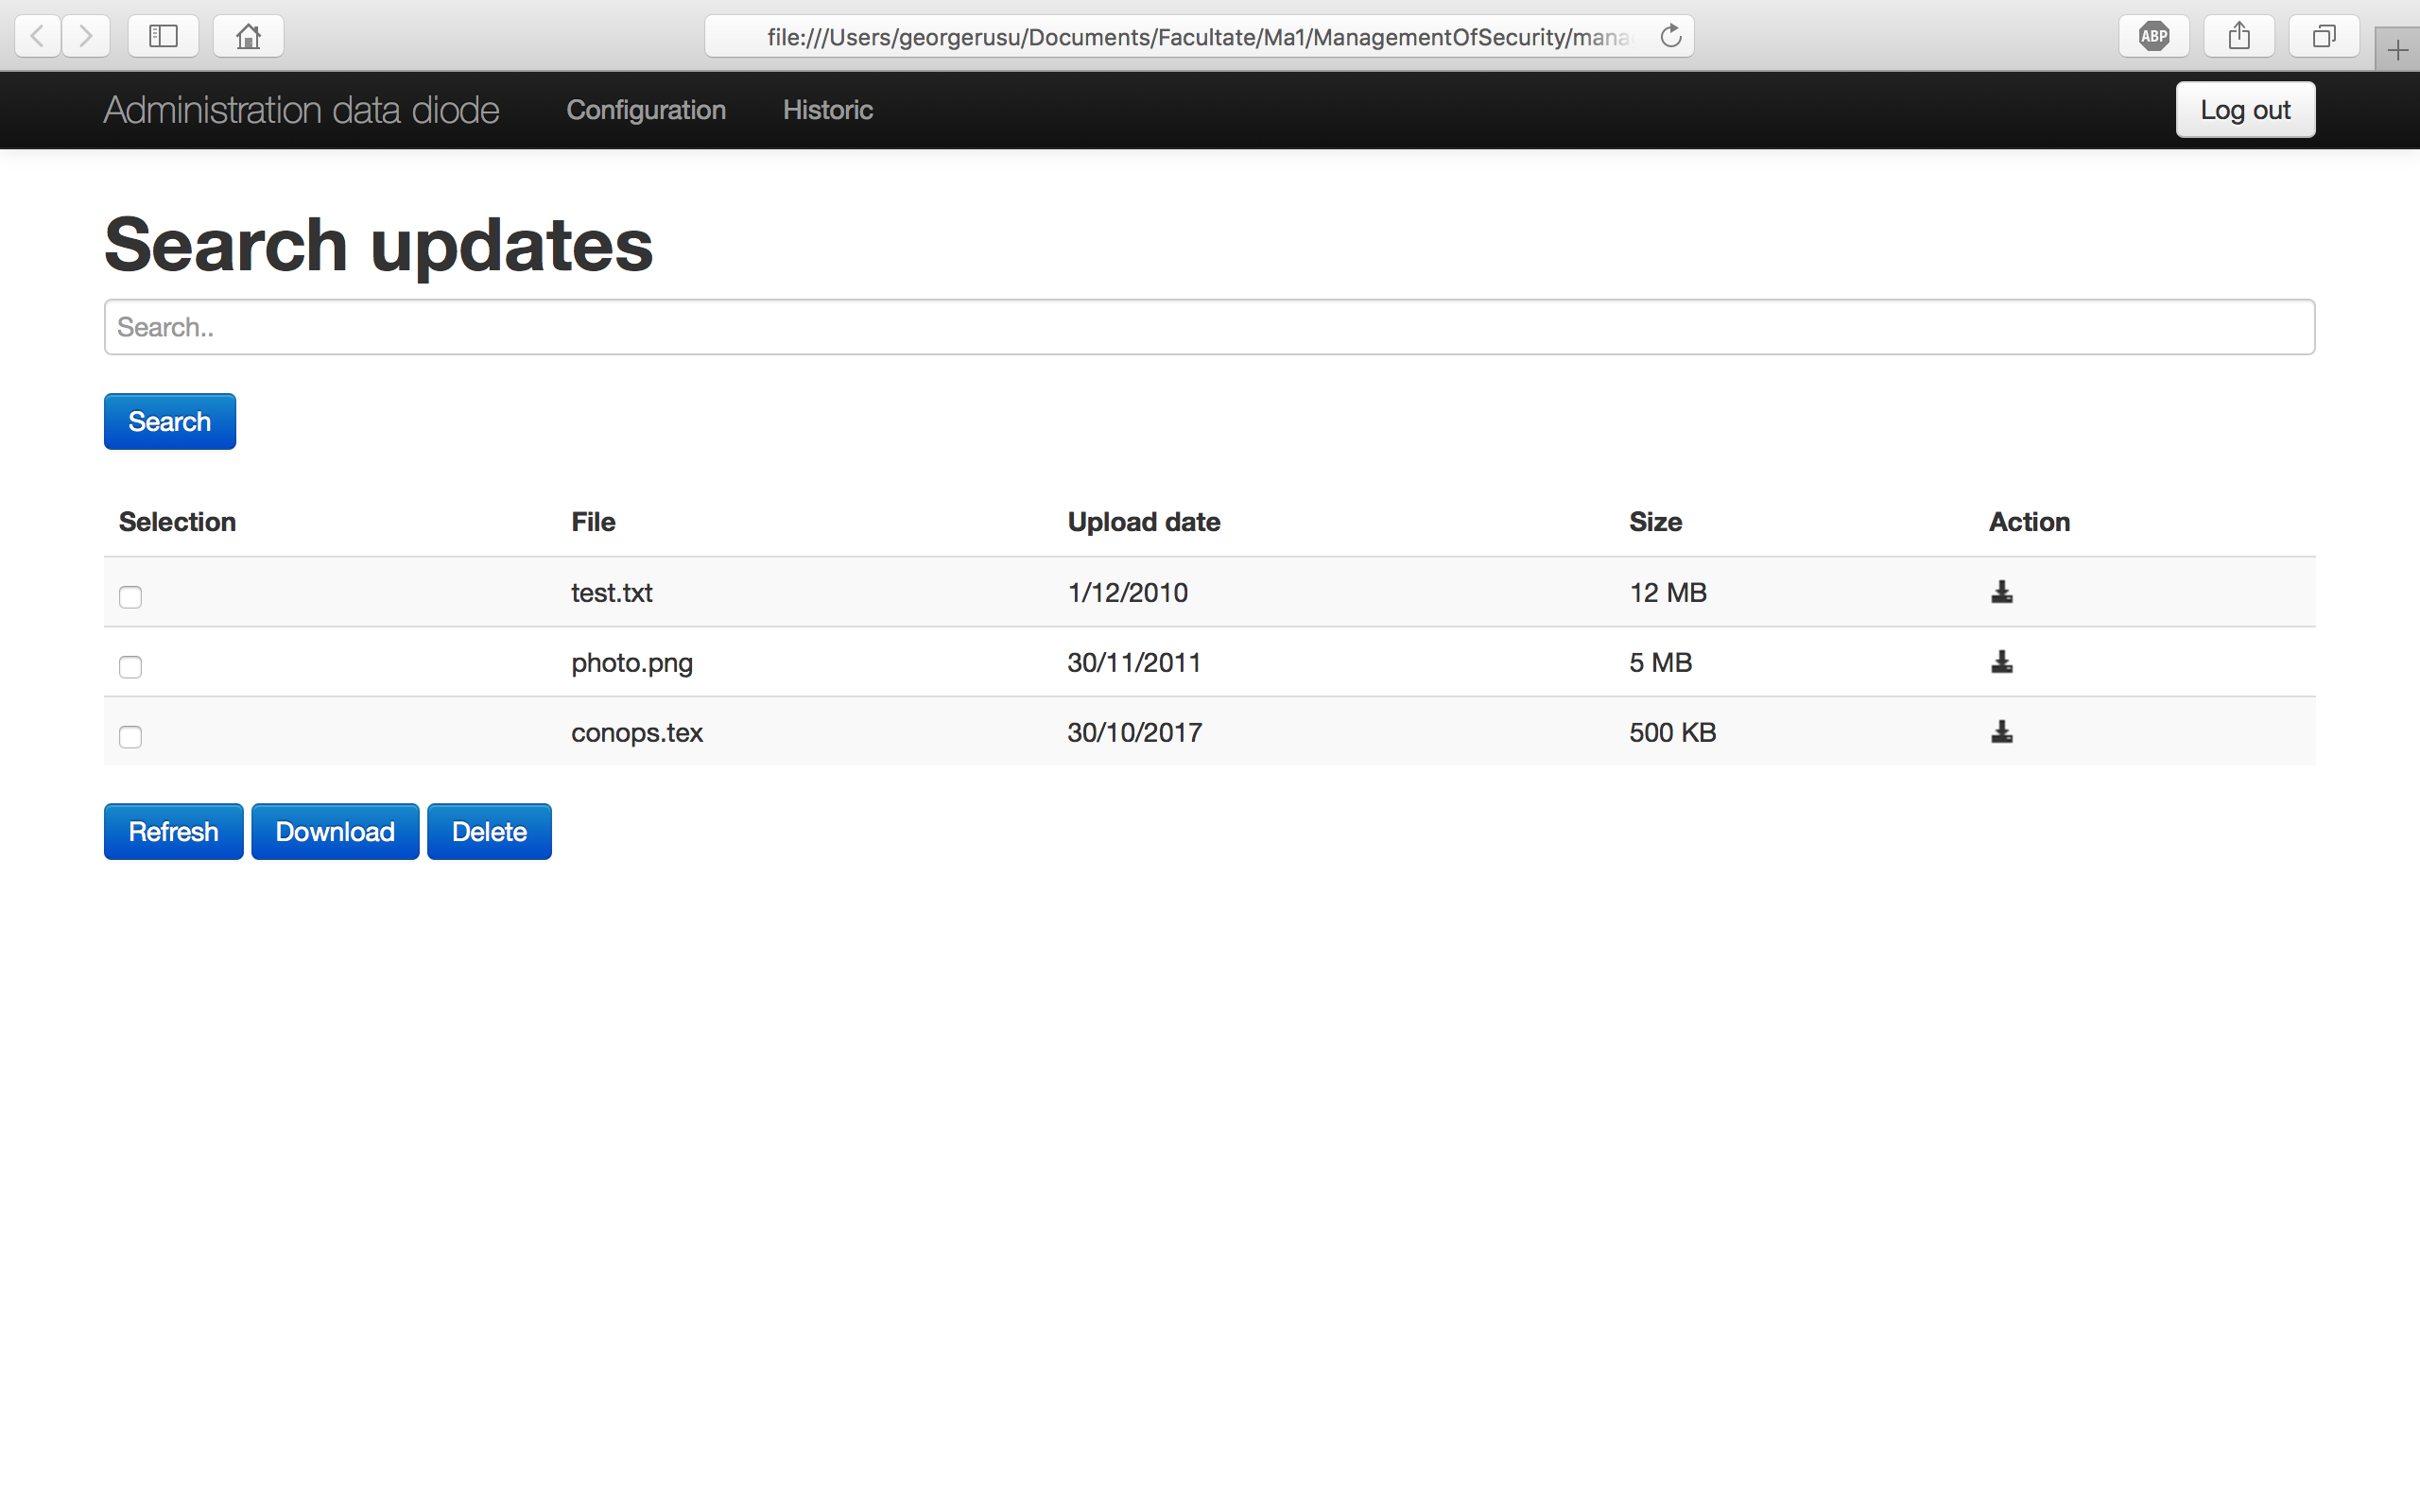
\includegraphics[scale=0.35]{images/adminreceiver.png}
\caption{Receiver admin page.}
\label{fig:receiveradminpage}
\end{figure}
\clearpage
\subsection{Usage of the WEB UI}
In this section we will explain how to use our web interfaces from different point of views.
\subsubsection{General usage}
In both cases, all users have to identify themselves through the login page with their credentials. They must fill in the form with their own username and password (Figure \ref{fig:logpage}). Once the form is submitted, the authentication will bring them respectively to their dedicated page.\bigskip 

In the case of a user connection, he will be redirected to the user transmission page according to his network location: if he is in the low security zone he will be prompted to use the transmission interface (Figure \ref{fig:transuserpage}) or he will get the receiver interface page (Figure \ref{fig:receiveruserpage}) if he stand on the high security zone (after the data diode). 

On the transmission page the user can select the files he needs and send them through the data diode by using the \textit{send} button. The user have also the possibility to upload a file from a computer and to add it in the selection list in order to transfer it. On the reception page, the user has a list of all the received files which he can depending on the button chosen and his selection, refresh, download or delete.\bigskip 

When an administrator will log in, similarly to the user mechanism, he will be redirected according to his network location : on the transmission interface or on the receiver interface, respectively Figure \ref{fig:transadminpage} and Figure \ref{fig:receiveradminpage}.

On the transmission page, a \textit{searchbar} is displayed to allow the administrator to search for available updates. He can search a specific update (button search) or display all available updates from officials repositories(button search all updates from sources). In this way he can select from a list the updates that he wants to transfer to the secure network. He can also upload files or new update packages from his computer. 

Furthermore, the administrator has an history page. With this page he can browse all the updates installed previously in the system  but he can also monitor all the passing data traffic between the two servers. This is made possible using a log information (user, date, size,...).

On the reception page, the administrator has access to all updates that have been send through the data diode. He can update all the machines using some Linux script or to use the web interface to download each update package manually on the desired machine and install them manually. Of course this manual method is not the most optimal but it could serve in case of a need for a system downgrade or an application downgrade on one workstation.

The administrators have the rights to manage all the updates within FTP sharing systems, they can choose to keep or delete updates.

\subsubsection{A Technical file transfer usage}
We have said earlier that their will be a web interface running on both side of the data diode. When a user will want to send a file, he would have to first login. The login page will use the data base of the company in order to authenticate users and to verify each one permissions. However, on the high security zone, the database would not be reachable because of the unidirectional data diode. Thus, once a user would want to send a file to the other side, there will be a daemon which will create a permission and ownership system in order for the other side to recognize to whom the file belongs to. For example, when the UserX would want to send the \emph{file.txt} to the other side, the daemon will rename the file using the following rule:
\begin{center}
\centering
\emph{file.txt} $\triangleright$ \emph{userName\_password\_fileName\_timestamp\_size\_extension.zip}
\end{center} 

Every file will be converted into a zip archive in order to reduce the initial size, thing that could sometimes have a major impact on the speed of the transfer (hence the time).\bigskip

On the other side, there will be of course another daemon which will for each file received, decompress the file into the original extension\footnote{This is why the initial extension is putted in to the name of the sent file.}. However to ensure that only the owner (thus the userName) may see the file, the second daemon will create for every userName a folder where received files will be stored. The rule for this operations is:
\begin{center}
\centering
\emph{userName\_password\_fileName\_timestamp\_size\_extension.zip} $\triangleright$ folder: \emph{userName\_password} $\triangleright$ files in folder: \emph{file.txt}
\end{center}

Furthermore, when a user wants to login from the secure zone of the data diode, instead of queering a database, the web interface will query a daemon which will use all the folders name to authenticate the user. Every password will not be shared in clear text, a hash of SHA-256 will be used. In this way there is no need of database duplication. The main verification will take place on the transmitter side where the database can be accessed: if a user has the permission to transfer a file, he will be able to transfer the file from the transmitter side. Thus, if the file is transmitted to the receiver side, it means that the user has an access granted on the security zone and thus he has already been verified. However, if a user has not yet used the transmission system of the data diode, he will not be able to connect to the interface from the receiver side.

\subsubsection{Configuration panel for the admin}

\begin{thebibliography}{9}


\bibitem{data-diode-work}
DEEP SECURE,
\textit{How	Does a Data Diode Work?}
Discussion Paper, February 2017.

\bibitem{data-diode-SANS-Institute}
SANS Institute InfoSec Reading Room,
\textit{Tactical Data Diodes in Industrial Automation and Control Systems}, January 2015.

\bibitem{data-diode-transport}
CS Risk Management and Compliance Ltd,
\textit{Data Diode vs Firewall Feasibility}, September 2016. [Online]. Available: \url{https://csriskmanagement.co.uk/data-diode-vs-firewall-feasibility/} [Accessed: 30- Oct- 2017]
\bibitem{data-diode-transport}

BlindFTP,
\textit{Blind ftp protocol}[Online]. Available: \url{https://www.decalage.info/fr/python/blindftp} [Accessed: 30- Oct- 2017]

\end{thebibliography}
\end{document}